\documentclass{X:/Documents/Coding/Latex/myassignment}
%%Document info
\title{OFN Assignment 5}
\begin{document}
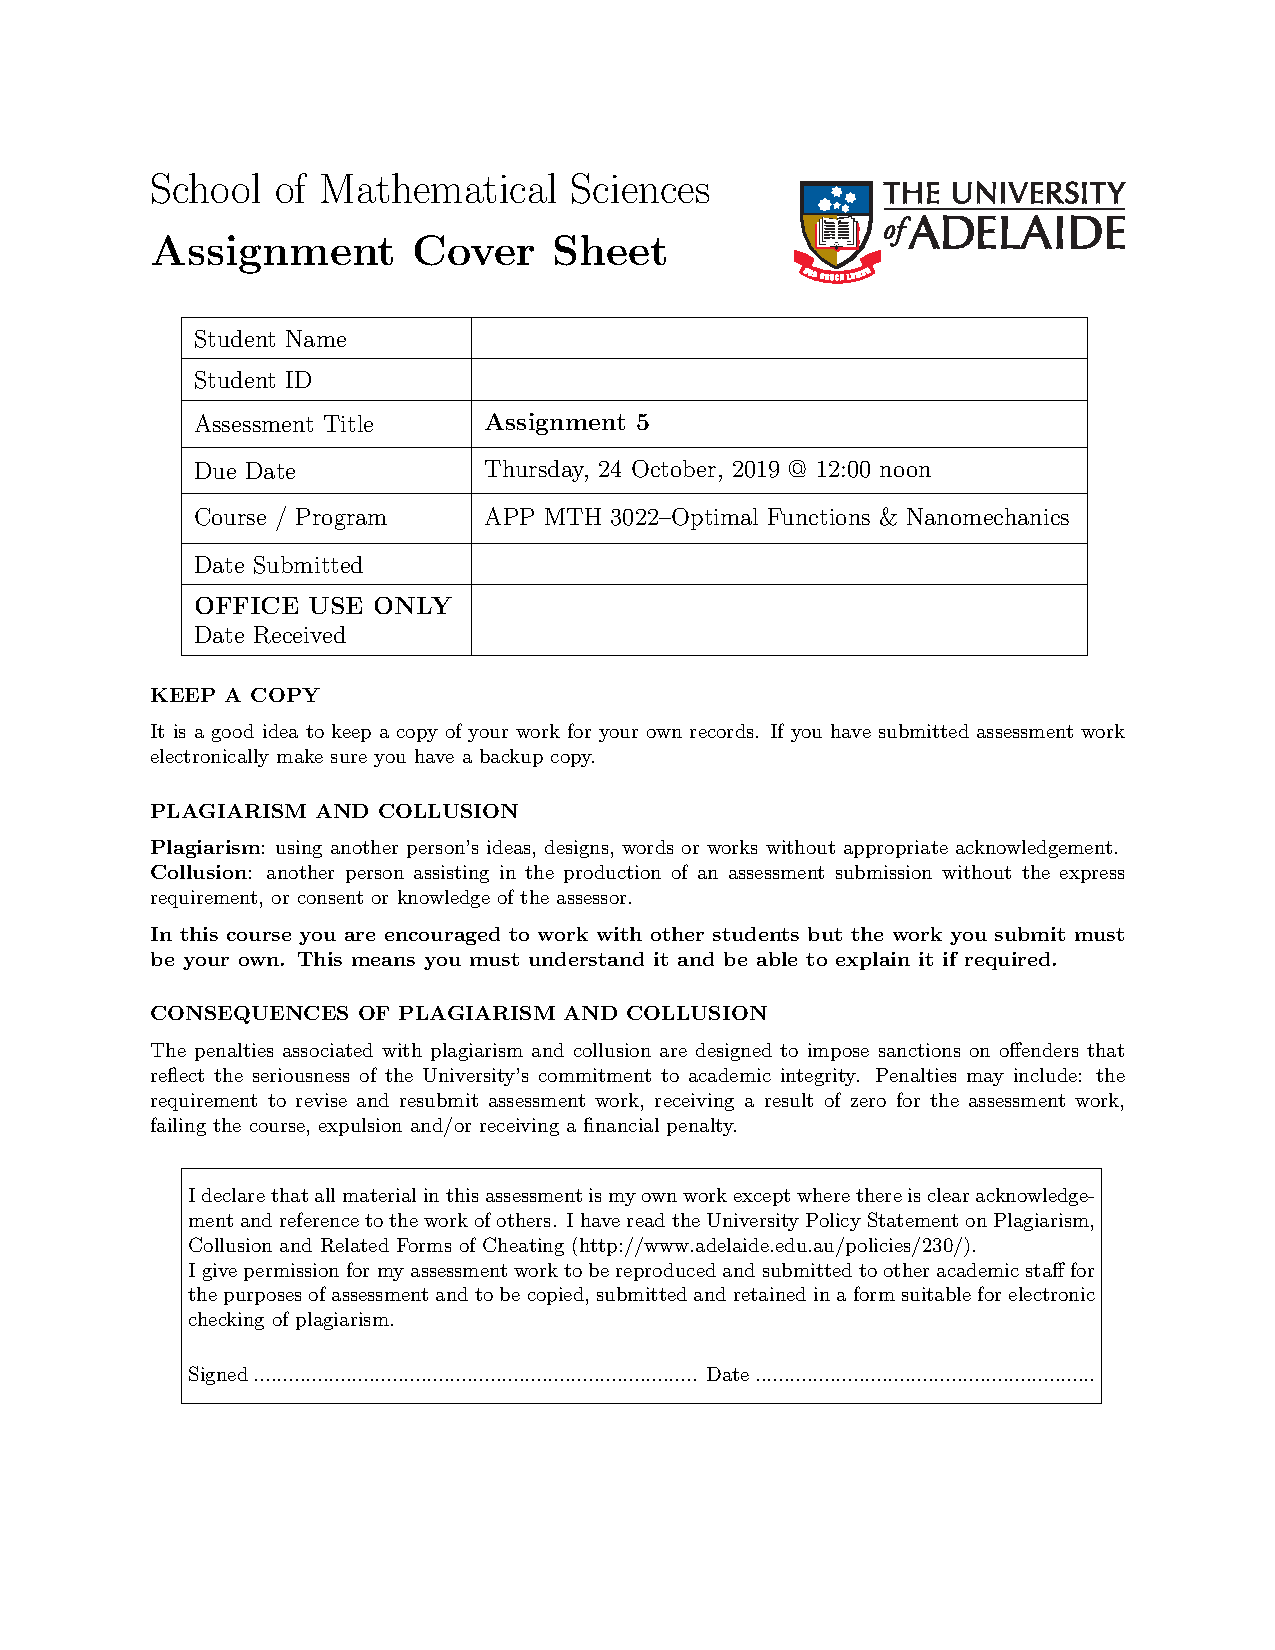
\includepdf{cover5}
\maketitle
\begin{enumerate}
	\item 
\begin{enumerate}
	\item Assume we are only considering the top surface of the substrate.
	\begin{enumerate}
		\item Area of the solid-liquid interface, $A_{sl}$:
		\[A_{sl} = \pi r_0^2\]
		\item Solid-gas interface, $A_{sg}$:

		This is the difference of the solid area and the solid liquid interface, that is:
		\[A_{sg} = A_s - A_{sl} = A_s - \pi r_0^2\]

		\item Liquid-gas interface, $A_{lg}$:

		This is the surface area of the droplet above the solid. The surface area of the droplet is parameterised as
		\[\vec r = \left(r(z)\cos u,r(z)\sin u,z\right)\]
		This is nearly to the soap film in assignment 4, the surface area of this becomes
		\begin{align*}
			S &= \int_{0}^{z_0} \int_{-\pi}^{\pi} r\sqrt{1+r'^2} dudz\\
			&= 2\pi  \int_{0}^{z_0} r\sqrt{1+r'^2} dz\\
		\end{align*}
		Which is the liquid-gas interface
		\[A_{lg} = S -A_{sl} = S \]
	\end{enumerate}
	\item Subbing all of the above into the total energy:
	\begin{align*}
		E_{tot} &= \gamma_{sl}\left(\pi r_0^2\right) + \gamma_{sg}\left(A_s - \pi r_0^2\right) + \gamma_{lg}S\\
		&= \gamma_{sl}\left(2\pi r_0\right) + \gamma_{sg}\left(A_s - \pi r_0^2\right) + \gamma_{lg}\left(2\pi \int_{0}^{z_0} r\sqrt{1+r'^2} dz\right)\\
	\end{align*}
	\item The volume of the droplet: cross sectional volume is just $dV = \pi r^2 dz$. 
	\begin{align*}
		V_l &= \int_0^{z_0}\pi r^2 dz\\
	\end{align*}

	That is the constraint is: 
	\[Constraint = - \pi \hat{\lambda} \int_0^{z_0} r^2 dz\]

	And hence the functional (which is no longer explicitly the energy) is
	\[F_1\{z\} = \gamma_{sl}\left(\pi r_0^2\right) + \gamma_{sg}\left(A_s - \pi r_0^2\right) + \gamma_{lg}\left(2\pi \left( \int_{0}^{z_0} r\sqrt{1+r'^2} - \lambda r^2 dz\right)\right)\]
	Where $\lambda = \frac{\hat{\lambda}}{2 \gamma_{lg}}$
	\item 
	\begin{align*}		
		F_2\{z\} &=  \gamma_{sl}\left(\pi r_0^2\right) + \gamma_{sg}\left(- \pi r_0^2\right) + \gamma_{lg}\left(2\pi \left( \int_{0}^{z_0} r\sqrt{1+r'^2} - \lambda r^2 dz\right)\right)\\
		F\{z\} &=\frac{1}{2\gamma_{lg}}\gamma_{sl}\left(r_0\right) + \frac{1}{2\gamma_{lg}}\gamma_{sg}\left(- r_0\right) + \left(\int_{0}^{z_0} r\sqrt{1+r'^2} - \lambda r^2 dz\right)\\		
		&= \left(\frac{\gamma_{sl} - \gamma_{sg}}{2 \gamma_{lg}} r_0^2 \right) + \int_0^{z_0} r\sqrt{1+r'^2} - \lambda r^2 dz\\
		&= \left[\left(\frac{\gamma_{sl} - \gamma_{sg}}{2 \gamma_{lg}}  \right)r^2\right]_{z=0} + \int_0^{z_0}\left( r\sqrt{1+r'^2} - \lambda r^2\right) dz
	\end{align*}
\end{enumerate}
	\item 
\begin{enumerate}
	\item 
	\begin{align*}
		p &= \dd f{r'} = \frac{rr'}{\sqrt{1+r'^2}}\\
		H &= \frac{rr'^2}{\sqrt{1+r'^2}} - \left(r\sqrt{1+r'^2} - \lambda r^2\right)\\
	\end{align*}
	\item Since there is no explicit dependence on the independent variable $z$, this is autonomous, and so the Hamiltonian is constant

	\item The natural BC at $z=z_0$ since this is first order is:
	\[\left[\dd f{r'}\right]_{z =z_0} = 0 \implies p|_{z=z_0} = 0\]
	
	Since $[p \delta r - H \delta z]_{z_0} = 0$
	This implies that $H \delta z\pipe_{z_0} = 0$
	and for non-trivial solutions this implies that $H$ is everywhere zero
	\item From $b,c$ we obtain
	\begin{align*}
		\frac{rr'^2}{\sqrt{1+r'^2}} - \left(r\sqrt{1+r'^2} - \lambda r^2\right) = 0
	\end{align*}
	\item 
	Solving the DE:
	\begin{align*}
		\frac{rr'^2}{\sqrt{1+r'^2}} - \left(r\sqrt{1+r'^2} - \lambda r^2\right) = 0\\
		rr'^2 - r(1+r'^2) - \lambda r^2 \sqrt{1 + r'^2} =0 \\
		-r + \lambda r^2 \sqrt{1+r'^2} = 0\\
		-1 + \lambda r \sqrt{1+r'^2} = 0\\
		r \sqrt{1+r'^2} = \frac{1}{\lambda}\\
		r'^2 = \frac{1}{\lambda^2 r^2} -1\\
		r' = \sqrt{\frac{1}{\lambda^2 r^2} -1}\\
	\end{align*}

	\begin{align*}
		\int \frac{1}{\sqrt{\frac{1}{\lambda^2 r^2} -1}} dr = \int dz
	\end{align*}
	The left integral:
	\begin{align*}
		\int \frac{1}{\sqrt{\frac{1}{\lambda^2 r^2} -1}} dr &=\lambda \int \frac{1}{\sqrt{\frac{1}{r^2} - \lambda^2 }} dr\\
		&=\lambda \int \frac{r}{\sqrt{1 - \lambda^2 r^2}} dr\\
		&= \lambda \int \frac{\sqrt{1 - \lambda^2 r^2}}{\lambda^2 r} \frac{r}{\sqrt{1 - \lambda^2 r^2}} dv\\&= \lambda \int  \frac{r}{\sqrt{1 - \lambda^2 r^2}} \frac{-\sqrt{1 - \lambda^2 r^2}}{\lambda^2 r}dv\\
		&= -\frac{1}{\lambda} \int dv\\
		&= -\frac{\sqrt{1 - \lambda^2 r^2}}{\lambda}  + const\\
	\end{align*}
	Where I have used the substitution
	\begin{align*}
		v &= \sqrt{1- \lambda^2 r^2}, \quad dv = \frac{-\sqrt{1- \lambda^2 r^2}}{\lambda^2 r}
	\end{align*}


	Plugging this back in:

	\begin{align*}
		\int \frac{1}{\sqrt{\frac{1}{\lambda^2 r^2} -1}} dr = \int dz\\
		-\frac{\sqrt{1 - \lambda^2 r^2}}{\lambda} &= z + c\\
		1 - \lambda^2 r^2 &= z^2 \lambda^2 + c \lambda^2 z + c \lambda^2\\
		\lambda^2 r^2 &= 1 - z^2 \lambda^2 - c \lambda^2 z - c \lambda^2\\
		r^2 &= \frac{1}{\lambda^2} - z^2 - c z - c\\
		r^2 &= \frac{1}{\lambda^2} - (z-c)^2\\
		(z-c)^2 + r^2 &= \frac{1}{\lambda^2}\\
		(z-c)^2 + r^2 &= R^2\\
	\end{align*}
	Where $R^2 = \frac{1}{\lambda^2}$
\end{enumerate}

	\item 
\begin{enumerate}
	\item The contact angle $\theta_c$ is defined as the angle inside the droplet tangential to its point of contact $(z,r) = (0,r_0)$. This is equivalent to the derivative of $r$ at $z=0$, i.e. $r'(z=0)$.

	Rewrite the solution for the droplet as
	\[r = \sqrt{R^2 - (z-c)^2}, \quad r' = -\frac{z-c}{R^2 - (z-c)^2} \]
	So that
	\[r_0 = \sqrt{R^2 - c^2}, \quad r'(z=0) = \theta_c = \frac{c}{r_0^2}\]
	\begin{align*}
		\frac{p}{r} &=  \frac{r'}{\sqrt{1+r'^2}}\\
		&=\frac{-\frac{z-c}{R^2 - (z-c)^2}}{\sqrt{1 + \left(\frac{z-c}{R^2 - (z-c)^2}\right)^2 }}\\
		\frac{p}{r}\pipe_{z=0} &=\frac{\frac{c}{R^2 - c^2}}{\sqrt{1 + \left(\frac{c}{R^2 - c^2}\right)^2 }}\\
		&= \frac{c}{r_0 \sqrt{1 + c^2/r_0^2}}\\
		&= \frac{c}{\sqrt{r_0^2 + c^2}}\\
	\end{align*}
	\begin{align*}
		\left(\frac{\gamma_{sl} - \gamma_{sg}}{\gamma_{lg}} \right)r - p =0\\
		\left(\frac{\gamma_{sl} - \gamma_{sg}}{\gamma_{lg}} \right)r -  \frac{rr'}{\sqrt{1+r'^2}}=0\\
		\left(\frac{\gamma_{sl} - \gamma_{sg}}{\gamma_{lg}} \right) -  \frac{r'}{\sqrt{1+r'^2}}=0\\
	\end{align*}
	At $z = 0$, use the derivative of $r$ in terms of $\theta_c$:
	If we use the parameterisation 
	\[\dd rz = \frac{\dd r\theta}{\dd z\theta} = - \frac{R\cos\theta}{R\sin\theta} = -\cot(\theta) \]
	Then 
	\begin{align*}
		r'|_{z=0} &= -\cot(\theta_c)\\
		\frac{r'}{1+r'^2} &= \frac{-\cot(\theta_c)}{\sqrt{1 +\cot^2(\theta_c)}}\\
		&= \frac{-\cot(\theta_c)}{\cosec(\theta_c)}\\
		&= \frac{-\cos(\theta_c)}{\sin(\theta_c)} \sin(\theta_c)\\
		&= -\cos(\theta_c)
	\end{align*}
	
	\begin{align*}
		\left(\frac{\gamma_{sl} - \gamma_{sg}}{\gamma_{lg}} \right) -  \frac{r'}{\sqrt{1+r'^2}}=0\\
		\left(\frac{\gamma_{sl} - \gamma_{sg}}{\gamma_{lg}} \right) - (-\cos(\theta_c))=0\\
		\gamma_{sl} - \gamma_{sg} = - \gamma_{lg}\cos(\theta_c)\\
		\gamma_{sg} - \gamma_{sl} =  \gamma_{lg}\cos(\theta_c)\\
	\end{align*}



	\item Letting
	\[z = c+R\cos\theta, \quad r = R\sin \theta\]
	
	\begin{align*}
		r' &= -\cot\theta = \frac{z-c}{r}\\
		r'|_{z=0} &= -\cot(\theta_c) = \frac{-c}{r_0}\\
		r_0 = c\tan(\theta_c)\\
	\end{align*}

	\begin{align*}
		z = 0 \implies c + R\cos\theta_c &= 0\\
		c &= - R\cos\theta_c
	\end{align*}

	Which can simplify the previous expression:
	\begin{align*}
		-\frac{\cos\theta_c}{\sin\theta_c} &= \frac{R\cos\theta_c}{r_0}\\
		-\frac{1}{\sin\theta_c} &= \frac{R}{r_0}\\
		r_0 &= - R\sin\theta_c
	\end{align*}
	% $\theta_c$ is obtained from the max value of $r$.
	% I.e. $\theta_c$ is the value obtained for $r'$ when $z=0$.
	% \begin{align*}
	% 	r' = R\cos\theta\\
	% \end{align*}
	% \begin{align*}
	% 	z = c + R\cos\theta\\
	% 	0 = c + r'\\
	% 	c = -\theta_c\\
	% \end{align*}

	% $r_0$ is $r$ for $z=0$, i.e. the solution to the system
	% \begin{align*}
	% c + R\cos\theta = 0\\
	% r_0 - R\sin\theta = 0
	% \end{align*}
	% So
	% \begin{align*}
	% 	\theta = \arccos\left(\frac{\theta_c}{R}\right)\\
	% 	\implies r_0 = R\sin \left( \arccos\left(\frac{\theta_c^2}{R^2}\right)\right)\\
	% 	\implies r_0 = R\sqrt{1 - \cos^2\arccos \frac{\theta_c^2}{R^2}}\\
	% 	\implies r_0 = R\sqrt{1 -\frac{\theta_c^2}{R^2}}\\
	% \end{align*}


	 \item The fixed volume constraint:
	 We will have to convert $z=0, z=z_0$ to theta points:
	 \begin{align*}
	 	z =0  &\implies  c - R\cos(\theta_0) = 0\\
	 	\theta_0 &= \arccos\left( \frac{c}{R}\right)\\
	 	&= \arccos\left( - R\cos\theta_c/R\right)\\
	 	&= \arccos\left(  - \cos\theta_c\right)\\
	 	&= \pi - \arccos\left(\cos\theta_c\right)\\
	 	\theta_0 &= \pi - \theta_c\\
	 \end{align*}
	 %\[z= 0 \implies c - \cos(\theta_0) = 0 \implies \theta_0= \arccos\left(\frac{\theta_c}{R}\right)\]
	 %\[z = z_0 \implies r = 0 \implies \theta = n\pi = 0\]

	 \begin{align*}
	 	z = z_0 \implies r = 0 \implies \theta_1 = n\pi = 0
	 \end{align*}

	 \begin{align*}
	 V_l &= \pi \int_{0}^{z_0} r^2 dz\\
	 	&= \pi \int_{\theta_0}^{\theta_1} r^2 \frac{dz}{d \theta} d\theta\\
	 	&= \pi \int_{\theta_0}^{0} R^2\sin^2\theta (-R\sin\theta) d\theta\\
	 	&= \pi \int_{0}^{\theta_0} R^3\sin^3\theta  d\theta\\
	 	&= \pi R^3 \int_{0}^{\theta_0} \sin^3\theta  d\theta\\
	 	&= \pi R^3 \left[\frac13 \cos^3 \theta -\cos\theta\right]_0^{\theta_0}\\
	 	V_l &= \pi R^3 \left(-\frac13 \cos^3 \theta_c +\cos\theta_c + \frac23\right)\\
	 	R^3 &= \frac{V_l}{\pi\left(-\frac13 \cos^3 \theta_c +\cos\theta_c + \frac23\right)}\\
	 	R &= \left(\frac{V_l}{\pi\left(-\frac13 \cos^3 \theta_c +\cos\theta_c + \frac23\right)}\right)^{1/3}\\
	 	% &= \pi R^3 \left(\frac13 \cos^3 \theta_0 -\cos\theta_0 - (\frac13  -1)\right)\\
	 	% &= \pi R^3 \left(\frac13 \left( \frac{\theta_c}{R}\right)^3 -\frac{\theta_c}{R} + \frac23\right)\\
	 	% &= \pi \left(\frac13 \theta_c^3 -R^2\theta_c + \frac23 R^3\right)\\
	 \end{align*}

	\item 
	So using the conditions:
	\begin{align*}
	 	R &= \left(\frac{V_l}{\pi\left(-\frac13 \cos^3 \theta_c +\cos\theta_c + \frac23\right)}\right)^{1/3}\\
		r_0 &= - R\sin\theta_c\\
		c &= - R\cos\theta_c
	\end{align*}
	Figure~\ref{fig:q3d} shows the plots of these solutions. They either indicate that no solutions exist in this region (unlikely) or that there is an error in previous working.
	\begin{figure}[tbh]
		\centering
		\includegraphics[width = 0.8\linewidth]{A5Q3d}
		\caption{Plot of the parameters against $\theta_c$.}
		\label{fig:q3d}
	\end{figure}
\end{enumerate}
\end{enumerate}
\section*{Code}
\lstinputlisting{A5Code.m}

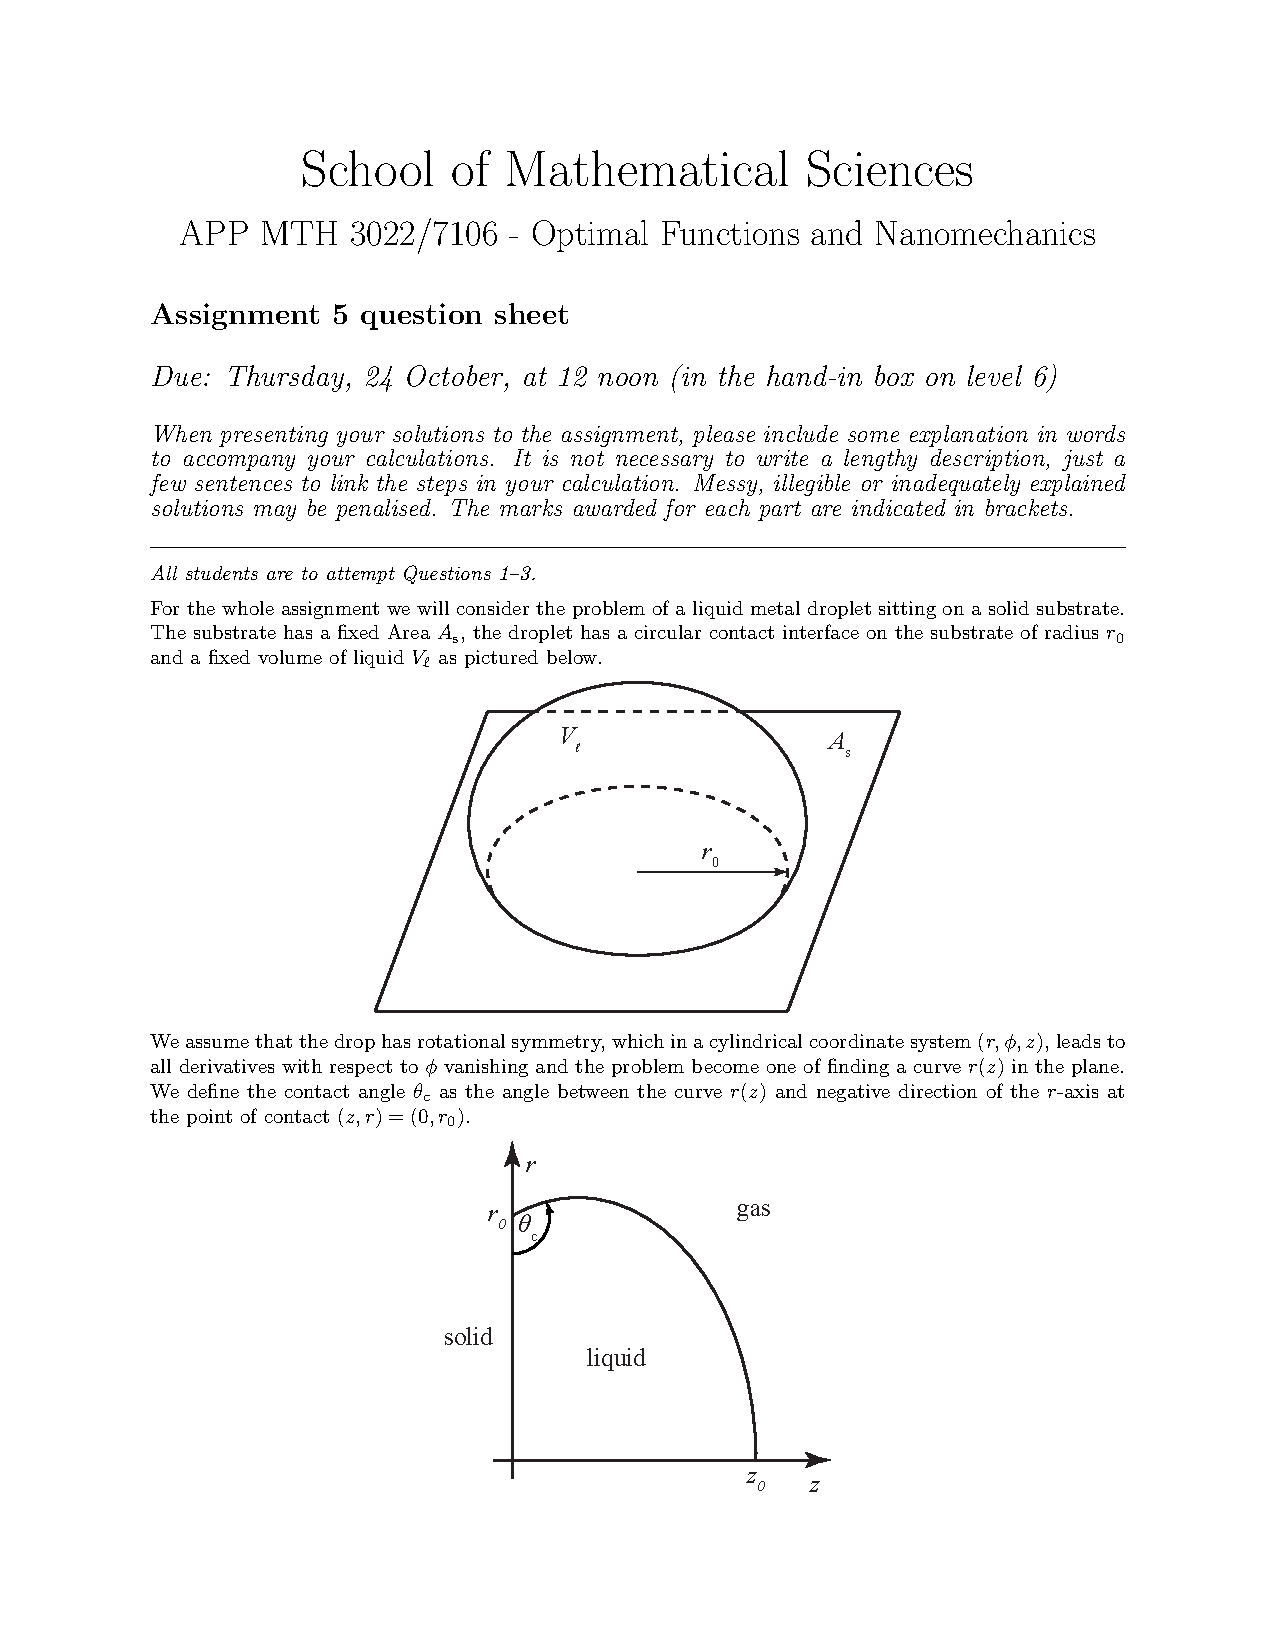
\includepdf[pages=1-]{assign5.pdf}

\end{document}